\chapter{Introduction}
\label{ch:introduction}
\section{Notations}
\label{sec:notations}
In this thesis, the following notations are used:
\begin{itemize}
  \item bold lowercase letters ($\vect{a}$, $\vect{b}$, $\vect{c}$) are used to denote vectors;
  \item italic lowercase letters ($a$, $b$, $c$) are used to denote scalars;
  \item bold uppercase letters ($\vect{A}$, $\vect{B}$, $\vect{C}$) are used to denote matrices;
\end{itemize}

No distinction in notation is made between a vector in the phisycal sense (applied to a point, with a direction, and a magnitude) and a vector in the mathematical sense (a generic number $\in \mathbb{R}^n $).

%\printinunitsof{in}\prntlen{\textwidth}

% \begin{figure*}
%   \centering
% \begin{subfigure}{0.3\linewidth}  % <----
%  % This file was created with tikzplotlib v0.10.1.
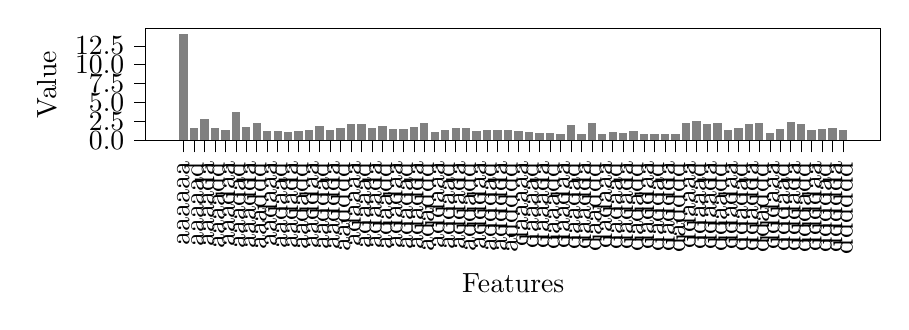
\begin{tikzpicture}

\definecolor{darkgray176}{RGB}{176,176,176}
\definecolor{gray}{RGB}{128,128,128}

\begin{axis}[
height=3cm,
tick align=outside,
tick pos=left,
width=0.9\linewidth,
x grid style={darkgray176},
xlabel={Features},
xmin=-3.59, xmax=66.59,
xtick style={color=black},
xtick={0,1,2,3,4,5,6,7,8,9,10,11,12,13,14,15,16,17,18,19,20,21,22,23,24,25,26,27,28,29,30,31,32,33,34,35,36,37,38,39,40,41,42,43,44,45,46,47,48,49,50,51,52,53,54,55,56,57,58,59,60,61,62,63},
xticklabel style={rotate=90.0},
xticklabels={
  aaaaaa,
  aaaaad,
  aaaada,
  aaaadd,
  aaadaa,
  aaadad,
  aaadda,
  aaaddd,
  aadaaa,
  aadaad,
  aadada,
  aadadd,
  aaddaa,
  aaddad,
  aaddda,
  aadddd,
  adaaaa,
  adaaad,
  adaada,
  adaadd,
  adadaa,
  adadad,
  adadda,
  adaddd,
  addaaa,
  addaad,
  addada,
  addadd,
  adddaa,
  adddad,
  adddda,
  addddd,
  daaaaa,
  daaaad,
  daaada,
  daaadd,
  daadaa,
  daadad,
  daadda,
  daaddd,
  dadaaa,
  dadaad,
  dadada,
  dadadd,
  daddaa,
  daddad,
  daddda,
  dadddd,
  ddaaaa,
  ddaaad,
  ddaada,
  ddaadd,
  ddadaa,
  ddadad,
  ddadda,
  ddaddd,
  dddaaa,
  dddaad,
  dddada,
  dddadd,
  ddddaa,
  ddddad,
  ddddda,
  dddddd
},
y grid style={darkgray176},
ylabel={Value},
ymin=0, ymax=14.7501854116883,
ytick style={color=black},
ytick={0,2.5,5,7.5,10,12.5,15},
yticklabels={
  \(\displaystyle {0.0}\),
  \(\displaystyle {2.5}\),
  \(\displaystyle {5.0}\),
  \(\displaystyle {7.5}\),
  \(\displaystyle {10.0}\),
  \(\displaystyle {12.5}\),
  \(\displaystyle {15.0}\)
}
]
\draw[draw=none,fill=gray] (axis cs:-0.4,0) rectangle (axis cs:0.4,14.0477956301794);
\draw[draw=none,fill=gray] (axis cs:0.6,0) rectangle (axis cs:1.4,1.58790560256716);
\draw[draw=none,fill=gray] (axis cs:1.6,0) rectangle (axis cs:2.4,2.81682594419133);
\draw[draw=none,fill=gray] (axis cs:2.6,0) rectangle (axis cs:3.4,1.68681511873817);
\draw[draw=none,fill=gray] (axis cs:3.6,0) rectangle (axis cs:4.4,1.33779456540034);
\draw[draw=none,fill=gray] (axis cs:4.6,0) rectangle (axis cs:5.4,3.72759670642379);
\draw[draw=none,fill=gray] (axis cs:5.6,0) rectangle (axis cs:6.4,1.7750517998814);
\draw[draw=none,fill=gray] (axis cs:6.6,0) rectangle (axis cs:7.4,2.30425289664694);
\draw[draw=none,fill=gray] (axis cs:7.6,0) rectangle (axis cs:8.4,1.23438263703416);
\draw[draw=none,fill=gray] (axis cs:8.6,0) rectangle (axis cs:9.4,1.23633291562529);
\draw[draw=none,fill=gray] (axis cs:9.6,0) rectangle (axis cs:10.4,1.09251292029537);
\draw[draw=none,fill=gray] (axis cs:10.6,0) rectangle (axis cs:11.4,1.28101619686892);
\draw[draw=none,fill=gray] (axis cs:11.6,0) rectangle (axis cs:12.4,1.40148015298769);
\draw[draw=none,fill=gray] (axis cs:12.6,0) rectangle (axis cs:13.4,1.87347846532573);
\draw[draw=none,fill=gray] (axis cs:13.6,0) rectangle (axis cs:14.4,1.33497528046836);
\draw[draw=none,fill=gray] (axis cs:14.6,0) rectangle (axis cs:15.4,1.6380019108117);
\draw[draw=none,fill=gray] (axis cs:15.6,0) rectangle (axis cs:16.4,2.23628653957849);
\draw[draw=none,fill=gray] (axis cs:16.6,0) rectangle (axis cs:17.4,2.16148392442204);
\draw[draw=none,fill=gray] (axis cs:17.6,0) rectangle (axis cs:18.4,1.66041273907827);
\draw[draw=none,fill=gray] (axis cs:18.6,0) rectangle (axis cs:19.4,1.85642911808637);
\draw[draw=none,fill=gray] (axis cs:19.6,0) rectangle (axis cs:20.4,1.4655850080051);
\draw[draw=none,fill=gray] (axis cs:20.6,0) rectangle (axis cs:21.4,1.48745776549568);
\draw[draw=none,fill=gray] (axis cs:21.6,0) rectangle (axis cs:22.4,1.77716331364945);
\draw[draw=none,fill=gray] (axis cs:22.6,0) rectangle (axis cs:23.4,2.24587006321554);
\draw[draw=none,fill=gray] (axis cs:23.6,0) rectangle (axis cs:24.4,1.17771959187167);
\draw[draw=none,fill=gray] (axis cs:24.6,0) rectangle (axis cs:25.4,1.39102644131561);
\draw[draw=none,fill=gray] (axis cs:25.6,0) rectangle (axis cs:26.4,1.62411269938688);
\draw[draw=none,fill=gray] (axis cs:26.6,0) rectangle (axis cs:27.4,1.60641302729228);
\draw[draw=none,fill=gray] (axis cs:27.6,0) rectangle (axis cs:28.4,1.27891803789233);
\draw[draw=none,fill=gray] (axis cs:28.6,0) rectangle (axis cs:29.4,1.33261293972183);
\draw[draw=none,fill=gray] (axis cs:29.6,0) rectangle (axis cs:30.4,1.43040484168112);
\draw[draw=none,fill=gray] (axis cs:30.6,0) rectangle (axis cs:31.4,1.38958373448553);
\draw[draw=none,fill=gray] (axis cs:31.6,0) rectangle (axis cs:32.4,1.31203428396195);
\draw[draw=none,fill=gray] (axis cs:32.6,0) rectangle (axis cs:33.4,1.15332496328426);
\draw[draw=none,fill=gray] (axis cs:33.6,0) rectangle (axis cs:34.4,1.01224747338895);
\draw[draw=none,fill=gray] (axis cs:34.6,0) rectangle (axis cs:35.4,0.998531518097484);
\draw[draw=none,fill=gray] (axis cs:35.6,0) rectangle (axis cs:36.4,0.809350332406363);
\draw[draw=none,fill=gray] (axis cs:36.6,0) rectangle (axis cs:37.4,1.97941164081068);
\draw[draw=none,fill=gray] (axis cs:37.6,0) rectangle (axis cs:38.4,0.90155293314939);
\draw[draw=none,fill=gray] (axis cs:38.6,0) rectangle (axis cs:39.4,2.28259299284546);
\draw[draw=none,fill=gray] (axis cs:39.6,0) rectangle (axis cs:40.4,0.899770228064936);
\draw[draw=none,fill=gray] (axis cs:40.6,0) rectangle (axis cs:41.4,1.15416615449955);
\draw[draw=none,fill=gray] (axis cs:41.6,0) rectangle (axis cs:42.4,1.02513659365138);
\draw[draw=none,fill=gray] (axis cs:42.6,0) rectangle (axis cs:43.4,1.30109732030214);
\draw[draw=none,fill=gray] (axis cs:43.6,0) rectangle (axis cs:44.4,0.810126417582991);
\draw[draw=none,fill=gray] (axis cs:44.6,0) rectangle (axis cs:45.4,0.900288302900823);
\draw[draw=none,fill=gray] (axis cs:45.6,0) rectangle (axis cs:46.4,0.844801306768224);
\draw[draw=none,fill=gray] (axis cs:46.6,0) rectangle (axis cs:47.4,0.810114956201998);
\draw[draw=none,fill=gray] (axis cs:47.6,0) rectangle (axis cs:48.4,2.28248655883471);
\draw[draw=none,fill=gray] (axis cs:48.6,0) rectangle (axis cs:49.4,2.53276182642304);
\draw[draw=none,fill=gray] (axis cs:49.6,0) rectangle (axis cs:50.4,2.22043972025534);
\draw[draw=none,fill=gray] (axis cs:50.6,0) rectangle (axis cs:51.4,2.36100583817908);
\draw[draw=none,fill=gray] (axis cs:51.6,0) rectangle (axis cs:52.4,1.37638015647527);
\draw[draw=none,fill=gray] (axis cs:52.6,0) rectangle (axis cs:53.4,1.70950934273352);
\draw[draw=none,fill=gray] (axis cs:53.6,0) rectangle (axis cs:54.4,2.1978839185094);
\draw[draw=none,fill=gray] (axis cs:54.6,0) rectangle (axis cs:55.4,2.34318957768077);
\draw[draw=none,fill=gray] (axis cs:55.6,0) rectangle (axis cs:56.4,1.0360168117102);
\draw[draw=none,fill=gray] (axis cs:56.6,0) rectangle (axis cs:57.4,1.51698986528462);
\draw[draw=none,fill=gray] (axis cs:57.6,0) rectangle (axis cs:58.4,2.44136370801308);
\draw[draw=none,fill=gray] (axis cs:58.6,0) rectangle (axis cs:59.4,2.21319244650176);
\draw[draw=none,fill=gray] (axis cs:59.6,0) rectangle (axis cs:60.4,1.40424374684726);
\draw[draw=none,fill=gray] (axis cs:60.6,0) rectangle (axis cs:61.4,1.46504849020539);
\draw[draw=none,fill=gray] (axis cs:61.6,0) rectangle (axis cs:62.4,1.66224972195976);
\draw[draw=none,fill=gray] (axis cs:62.6,0) rectangle (axis cs:63.4,1.31624861899134);
\end{axis}

\end{tikzpicture}

%  \caption{Model 1}
%  \label{fig1a}
% \end{subfigure}

% \begin{subfigure}{0.3\linewidth}  % <----
%  % This file was created with tikzplotlib v0.10.1.
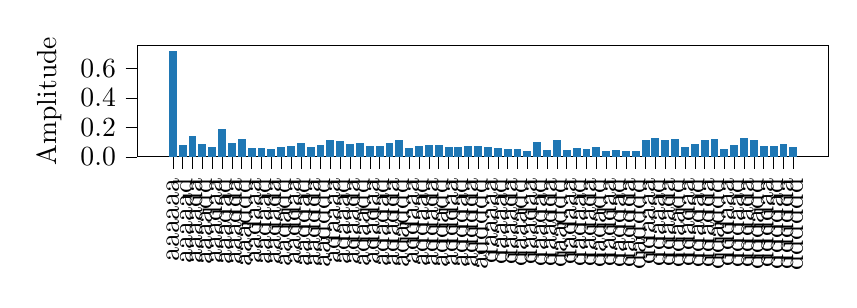
\begin{tikzpicture}

\definecolor{darkgray176}{RGB}{176,176,176}
\definecolor{steelblue31119180}{RGB}{31,119,180}

\begin{axis}[
height=3cm,
tick align=outside,
tick pos=left,
width=294.76926pt,
x grid style={darkgray176},
xmin=-3.59, xmax=66.59,
xtick style={color=black},
xtick={0,1,2,3,4,5,6,7,8,9,10,11,12,13,14,15,16,17,18,19,20,21,22,23,24,25,26,27,28,29,30,31,32,33,34,35,36,37,38,39,40,41,42,43,44,45,46,47,48,49,50,51,52,53,54,55,56,57,58,59,60,61,62,63},
xticklabel style={rotate=90.0},
xticklabels={
  aaaaaa,
  aaaaad,
  aaaada,
  aaaadd,
  aaadaa,
  aaadad,
  aaadda,
  aaaddd,
  aadaaa,
  aadaad,
  aadada,
  aadadd,
  aaddaa,
  aaddad,
  aaddda,
  aadddd,
  adaaaa,
  adaaad,
  adaada,
  adaadd,
  adadaa,
  adadad,
  adadda,
  adaddd,
  addaaa,
  addaad,
  addada,
  addadd,
  adddaa,
  adddad,
  adddda,
  addddd,
  daaaaa,
  daaaad,
  daaada,
  daaadd,
  daadaa,
  daadad,
  daadda,
  daaddd,
  dadaaa,
  dadaad,
  dadada,
  dadadd,
  daddaa,
  daddad,
  daddda,
  dadddd,
  ddaaaa,
  ddaaad,
  ddaada,
  ddaadd,
  ddadaa,
  ddadad,
  ddadda,
  ddaddd,
  dddaaa,
  dddaad,
  dddada,
  dddadd,
  ddddaa,
  ddddad,
  ddddda,
  dddddd
},
y grid style={darkgray176},
ylabel={Amplitude},
ymin=0, ymax=0.758179630791467,
ytick style={color=black},
ytick={0,0.2,0.4,0.6,0.8},
yticklabels={
  \(\displaystyle {0.0}\),
  \(\displaystyle {0.2}\),
  \(\displaystyle {0.4}\),
  \(\displaystyle {0.6}\),
  \(\displaystyle {0.8}\)
}
]
\draw[draw=none,fill=steelblue31119180] (axis cs:-0.4,0) rectangle (axis cs:0.4,0.722075838849016);
\draw[draw=none,fill=steelblue31119180] (axis cs:0.6,0) rectangle (axis cs:1.4,0.0816205118704516);
\draw[draw=none,fill=steelblue31119180] (axis cs:1.6,0) rectangle (axis cs:2.4,0.144788692125759);
\draw[draw=none,fill=steelblue31119180] (axis cs:2.6,0) rectangle (axis cs:3.4,0.0867045957893479);
\draw[draw=none,fill=steelblue31119180] (axis cs:3.6,0) rectangle (axis cs:4.4,0.0687644637243896);
\draw[draw=none,fill=steelblue31119180] (axis cs:4.6,0) rectangle (axis cs:5.4,0.191603550445973);
\draw[draw=none,fill=steelblue31119180] (axis cs:5.6,0) rectangle (axis cs:6.4,0.0912400814435433);
\draw[draw=none,fill=steelblue31119180] (axis cs:6.6,0) rectangle (axis cs:7.4,0.118441738979468);
\draw[draw=none,fill=steelblue31119180] (axis cs:7.6,0) rectangle (axis cs:8.4,0.063448949683056);
\draw[draw=none,fill=steelblue31119180] (axis cs:8.6,0) rectangle (axis cs:9.4,0.063549196660358);
\draw[draw=none,fill=steelblue31119180] (axis cs:9.6,0) rectangle (axis cs:10.4,0.0561566529115002);
\draw[draw=none,fill=steelblue31119180] (axis cs:10.6,0) rectangle (axis cs:11.4,0.0658459782078631);
\draw[draw=none,fill=steelblue31119180] (axis cs:11.6,0) rectangle (axis cs:12.4,0.0720379897131174);
\draw[draw=none,fill=steelblue31119180] (axis cs:12.6,0) rectangle (axis cs:13.4,0.0962993461770895);
\draw[draw=none,fill=steelblue31119180] (axis cs:13.6,0) rectangle (axis cs:14.4,0.0686195486369405);
\draw[draw=none,fill=steelblue31119180] (axis cs:14.6,0) rectangle (axis cs:15.4,0.0841955303823389);
\draw[draw=none,fill=steelblue31119180] (axis cs:15.6,0) rectangle (axis cs:16.4,0.114948175605847);
\draw[draw=none,fill=steelblue31119180] (axis cs:16.6,0) rectangle (axis cs:17.4,0.111103219250477);
\draw[draw=none,fill=steelblue31119180] (axis cs:17.6,0) rectangle (axis cs:18.4,0.0853474774953162);
\draw[draw=none,fill=steelblue31119180] (axis cs:18.6,0) rectangle (axis cs:19.4,0.0954229864952013);
\draw[draw=none,fill=steelblue31119180] (axis cs:19.6,0) rectangle (axis cs:20.4,0.0753330666191015);
\draw[draw=none,fill=steelblue31119180] (axis cs:20.6,0) rectangle (axis cs:21.4,0.0764573561609443);
\draw[draw=none,fill=steelblue31119180] (axis cs:21.6,0) rectangle (axis cs:22.4,0.0913486161286602);
\draw[draw=none,fill=steelblue31119180] (axis cs:22.6,0) rectangle (axis cs:23.4,0.115440781780618);
\draw[draw=none,fill=steelblue31119180] (axis cs:23.6,0) rectangle (axis cs:24.4,0.0605363919448476);
\draw[draw=none,fill=steelblue31119180] (axis cs:24.6,0) rectangle (axis cs:25.4,0.0715006546875076);
\draw[draw=none,fill=steelblue31119180] (axis cs:25.6,0) rectangle (axis cs:26.4,0.0834816059877538);
\draw[draw=none,fill=steelblue31119180] (axis cs:26.6,0) rectangle (axis cs:27.4,0.0825718187220844);
\draw[draw=none,fill=steelblue31119180] (axis cs:27.6,0) rectangle (axis cs:28.4,0.0657381299772261);
\draw[draw=none,fill=steelblue31119180] (axis cs:28.6,0) rectangle (axis cs:29.4,0.0684981211033183);
\draw[draw=none,fill=steelblue31119180] (axis cs:29.6,0) rectangle (axis cs:30.4,0.0735247581287173);
\draw[draw=none,fill=steelblue31119180] (axis cs:30.6,0) rectangle (axis cs:31.4,0.0714264975904106);
\draw[draw=none,fill=steelblue31119180] (axis cs:31.6,0) rectangle (axis cs:32.4,0.0674403501539547);
\draw[draw=none,fill=steelblue31119180] (axis cs:32.6,0) rectangle (axis cs:33.4,0.0592824747919798);
\draw[draw=none,fill=steelblue31119180] (axis cs:33.6,0) rectangle (axis cs:34.4,0.052030899559776);
\draw[draw=none,fill=steelblue31119180] (axis cs:34.6,0) rectangle (axis cs:35.4,0.0513258807665482);
\draw[draw=none,fill=steelblue31119180] (axis cs:35.6,0) rectangle (axis cs:36.4,0.0416017100177299);
\draw[draw=none,fill=steelblue31119180] (axis cs:36.6,0) rectangle (axis cs:37.4,0.101744455756126);
\draw[draw=none,fill=steelblue31119180] (axis cs:37.6,0) rectangle (axis cs:38.4,0.0463410493438625);
\draw[draw=none,fill=steelblue31119180] (axis cs:38.6,0) rectangle (axis cs:39.4,0.117328390407309);
\draw[draw=none,fill=steelblue31119180] (axis cs:39.6,0) rectangle (axis cs:40.4,0.0462494158731625);
\draw[draw=none,fill=steelblue31119180] (axis cs:40.6,0) rectangle (axis cs:41.4,0.0593257131667686);
\draw[draw=none,fill=steelblue31119180] (axis cs:41.6,0) rectangle (axis cs:42.4,0.0526934179057522);
\draw[draw=none,fill=steelblue31119180] (axis cs:42.6,0) rectangle (axis cs:43.4,0.0668781753176304);
\draw[draw=none,fill=steelblue31119180] (axis cs:43.6,0) rectangle (axis cs:44.4,0.0416416018534089);
\draw[draw=none,fill=steelblue31119180] (axis cs:44.6,0) rectangle (axis cs:45.4,0.0462760456257271);
\draw[draw=none,fill=steelblue31119180] (axis cs:45.6,0) rectangle (axis cs:46.4,0.0434239384103015);
\draw[draw=none,fill=steelblue31119180] (axis cs:46.6,0) rectangle (axis cs:47.4,0.0416410127228071);
\draw[draw=none,fill=steelblue31119180] (axis cs:47.6,0) rectangle (axis cs:48.4,0.117322919554115);
\draw[draw=none,fill=steelblue31119180] (axis cs:48.6,0) rectangle (axis cs:49.4,0.130187409367646);
\draw[draw=none,fill=steelblue31119180] (axis cs:49.6,0) rectangle (axis cs:50.4,0.114133627497582);
\draw[draw=none,fill=steelblue31119180] (axis cs:50.6,0) rectangle (axis cs:51.4,0.121358917513582);
\draw[draw=none,fill=steelblue31119180] (axis cs:51.6,0) rectangle (axis cs:52.4,0.0707478156876725);
\draw[draw=none,fill=steelblue31119180] (axis cs:52.6,0) rectangle (axis cs:53.4,0.0878711098289786);
\draw[draw=none,fill=steelblue31119180] (axis cs:53.6,0) rectangle (axis cs:54.4,0.112974228550204);
\draw[draw=none,fill=steelblue31119180] (axis cs:54.6,0) rectangle (axis cs:55.4,0.120443137445082);
\draw[draw=none,fill=steelblue31119180] (axis cs:55.6,0) rectangle (axis cs:56.4,0.053252675940857);
\draw[draw=none,fill=steelblue31119180] (axis cs:56.6,0) rectangle (axis cs:57.4,0.077975346334595);
\draw[draw=none,fill=steelblue31119180] (axis cs:57.6,0) rectangle (axis cs:58.4,0.125489421529731);
\draw[draw=none,fill=steelblue31119180] (axis cs:58.6,0) rectangle (axis cs:59.4,0.113761107750516);
\draw[draw=none,fill=steelblue31119180] (axis cs:59.6,0) rectangle (axis cs:60.4,0.0721800422035524);
\draw[draw=none,fill=steelblue31119180] (axis cs:60.6,0) rectangle (axis cs:61.4,0.0753054888730634);
\draw[draw=none,fill=steelblue31119180] (axis cs:61.6,0) rectangle (axis cs:62.4,0.0854419009187501);
\draw[draw=none,fill=steelblue31119180] (axis cs:62.6,0) rectangle (axis cs:63.4,0.0676569727174981);
\end{axis}

\end{tikzpicture}

%  \caption{Model 2}
%  \label{fig1b}
% \end{subfigure}

% \begin{subfigure}{0.3\linewidth}  % <----
%  % This file was created with tikzplotlib v0.10.1.
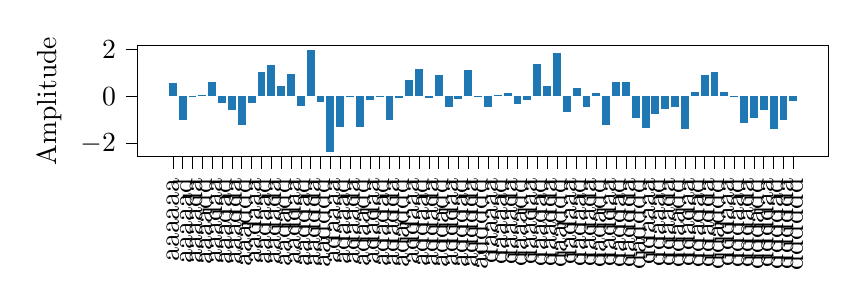
\begin{tikzpicture}

\definecolor{darkgray176}{RGB}{176,176,176}
\definecolor{steelblue31119180}{RGB}{31,119,180}

\begin{axis}[
height=3cm,
tick align=outside,
tick pos=left,
width=294.76926pt,
x grid style={darkgray176},
xmin=-3.59, xmax=66.59,
xtick style={color=black},
xtick={0,1,2,3,4,5,6,7,8,9,10,11,12,13,14,15,16,17,18,19,20,21,22,23,24,25,26,27,28,29,30,31,32,33,34,35,36,37,38,39,40,41,42,43,44,45,46,47,48,49,50,51,52,53,54,55,56,57,58,59,60,61,62,63},
xticklabel style={rotate=90.0},
xticklabels={
  aaaaaa,
  aaaaad,
  aaaada,
  aaaadd,
  aaadaa,
  aaadad,
  aaadda,
  aaaddd,
  aadaaa,
  aadaad,
  aadada,
  aadadd,
  aaddaa,
  aaddad,
  aaddda,
  aadddd,
  adaaaa,
  adaaad,
  adaada,
  adaadd,
  adadaa,
  adadad,
  adadda,
  adaddd,
  addaaa,
  addaad,
  addada,
  addadd,
  adddaa,
  adddad,
  adddda,
  addddd,
  daaaaa,
  daaaad,
  daaada,
  daaadd,
  daadaa,
  daadad,
  daadda,
  daaddd,
  dadaaa,
  dadaad,
  dadada,
  dadadd,
  daddaa,
  daddad,
  daddda,
  dadddd,
  ddaaaa,
  ddaaad,
  ddaada,
  ddaadd,
  ddadaa,
  ddadad,
  ddadda,
  ddaddd,
  dddaaa,
  dddaad,
  dddada,
  dddadd,
  ddddaa,
  ddddad,
  ddddda,
  dddddd
},
y grid style={darkgray176},
ylabel={Amplitude},
ymin=-2.57970469558561, ymax=2.17995924752535,
ytick style={color=black},
ytick={-4,-2,0,2,4},
yticklabels={
  \(\displaystyle {\ensuremath{-}4}\),
  \(\displaystyle {\ensuremath{-}2}\),
  \(\displaystyle {0}\),
  \(\displaystyle {2}\),
  \(\displaystyle {4}\)
}
]
\draw[draw=none,fill=steelblue31119180] (axis cs:-0.4,0) rectangle (axis cs:0.4,0.56400715619097);
\draw[draw=none,fill=steelblue31119180] (axis cs:0.6,0) rectangle (axis cs:1.4,-0.99045393478315);
\draw[draw=none,fill=steelblue31119180] (axis cs:1.6,0) rectangle (axis cs:2.4,-0.0198162012202089);
\draw[draw=none,fill=steelblue31119180] (axis cs:2.6,0) rectangle (axis cs:3.4,0.0624530588631012);
\draw[draw=none,fill=steelblue31119180] (axis cs:3.6,0) rectangle (axis cs:4.4,0.633698424314258);
\draw[draw=none,fill=steelblue31119180] (axis cs:4.6,0) rectangle (axis cs:5.4,-0.291680375891109);
\draw[draw=none,fill=steelblue31119180] (axis cs:5.6,0) rectangle (axis cs:6.4,-0.592403532321137);
\draw[draw=none,fill=steelblue31119180] (axis cs:6.6,0) rectangle (axis cs:7.4,-1.22388518360523);
\draw[draw=none,fill=steelblue31119180] (axis cs:7.6,0) rectangle (axis cs:8.4,-0.264577289250222);
\draw[draw=none,fill=steelblue31119180] (axis cs:8.6,0) rectangle (axis cs:9.4,1.02261380328961);
\draw[draw=none,fill=steelblue31119180] (axis cs:9.6,0) rectangle (axis cs:10.4,1.35655254507443);
\draw[draw=none,fill=steelblue31119180] (axis cs:10.6,0) rectangle (axis cs:11.4,0.459939265122322);
\draw[draw=none,fill=steelblue31119180] (axis cs:11.6,0) rectangle (axis cs:12.4,0.943889159786297);
\draw[draw=none,fill=steelblue31119180] (axis cs:12.6,0) rectangle (axis cs:13.4,-0.428999800592448);
\draw[draw=none,fill=steelblue31119180] (axis cs:13.6,0) rectangle (axis cs:14.4,1.96361088647485);
\draw[draw=none,fill=steelblue31119180] (axis cs:14.6,0) rectangle (axis cs:15.4,-0.252138127264008);
\draw[draw=none,fill=steelblue31119180] (axis cs:15.6,0) rectangle (axis cs:16.4,-2.36335633453511);
\draw[draw=none,fill=steelblue31119180] (axis cs:16.6,0) rectangle (axis cs:17.4,-1.29907274542126);
\draw[draw=none,fill=steelblue31119180] (axis cs:17.6,0) rectangle (axis cs:18.4,-0.0219003097275746);
\draw[draw=none,fill=steelblue31119180] (axis cs:18.6,0) rectangle (axis cs:19.4,-1.31350517091445);
\draw[draw=none,fill=steelblue31119180] (axis cs:19.6,0) rectangle (axis cs:20.4,-0.151642902118611);
\draw[draw=none,fill=steelblue31119180] (axis cs:20.6,0) rectangle (axis cs:21.4,-0.0401725057449436);
\draw[draw=none,fill=steelblue31119180] (axis cs:21.6,0) rectangle (axis cs:22.4,-0.991729597925402);
\draw[draw=none,fill=steelblue31119180] (axis cs:22.6,0) rectangle (axis cs:23.4,-0.0637959531300138);
\draw[draw=none,fill=steelblue31119180] (axis cs:23.6,0) rectangle (axis cs:24.4,0.712178268493982);
\draw[draw=none,fill=steelblue31119180] (axis cs:24.6,0) rectangle (axis cs:25.4,1.17720643151094);
\draw[draw=none,fill=steelblue31119180] (axis cs:25.6,0) rectangle (axis cs:26.4,-0.0681476201279612);
\draw[draw=none,fill=steelblue31119180] (axis cs:26.6,0) rectangle (axis cs:27.4,0.918376029178712);
\draw[draw=none,fill=steelblue31119180] (axis cs:27.6,0) rectangle (axis cs:28.4,-0.439271526522302);
\draw[draw=none,fill=steelblue31119180] (axis cs:28.6,0) rectangle (axis cs:29.4,-0.104443817954518);
\draw[draw=none,fill=steelblue31119180] (axis cs:29.6,0) rectangle (axis cs:30.4,1.11841844275852);
\draw[draw=none,fill=steelblue31119180] (axis cs:30.6,0) rectangle (axis cs:31.4,-0.0116538777843809);
\draw[draw=none,fill=steelblue31119180] (axis cs:31.6,0) rectangle (axis cs:32.4,-0.453067685094026);
\draw[draw=none,fill=steelblue31119180] (axis cs:32.6,0) rectangle (axis cs:33.4,0.0418960823419985);
\draw[draw=none,fill=steelblue31119180] (axis cs:33.6,0) rectangle (axis cs:34.4,0.151139857640656);
\draw[draw=none,fill=steelblue31119180] (axis cs:34.6,0) rectangle (axis cs:35.4,-0.335107310024924);
\draw[draw=none,fill=steelblue31119180] (axis cs:35.6,0) rectangle (axis cs:36.4,-0.14480730118177);
\draw[draw=none,fill=steelblue31119180] (axis cs:36.6,0) rectangle (axis cs:37.4,1.3921526991207);
\draw[draw=none,fill=steelblue31119180] (axis cs:37.6,0) rectangle (axis cs:38.4,0.437177994790058);
\draw[draw=none,fill=steelblue31119180] (axis cs:38.6,0) rectangle (axis cs:39.4,1.83139984658961);
\draw[draw=none,fill=steelblue31119180] (axis cs:39.6,0) rectangle (axis cs:40.4,-0.686238403562816);
\draw[draw=none,fill=steelblue31119180] (axis cs:40.6,0) rectangle (axis cs:41.4,0.337065328127374);
\draw[draw=none,fill=steelblue31119180] (axis cs:41.6,0) rectangle (axis cs:42.4,-0.438159895523348);
\draw[draw=none,fill=steelblue31119180] (axis cs:42.6,0) rectangle (axis cs:43.4,0.139733411042586);
\draw[draw=none,fill=steelblue31119180] (axis cs:43.6,0) rectangle (axis cs:44.4,-1.218864867566);
\draw[draw=none,fill=steelblue31119180] (axis cs:44.6,0) rectangle (axis cs:45.4,0.62702757250201);
\draw[draw=none,fill=steelblue31119180] (axis cs:45.6,0) rectangle (axis cs:46.4,0.627317437098576);
\draw[draw=none,fill=steelblue31119180] (axis cs:46.6,0) rectangle (axis cs:47.4,-0.939738712920593);
\draw[draw=none,fill=steelblue31119180] (axis cs:47.6,0) rectangle (axis cs:48.4,-1.34110547983178);
\draw[draw=none,fill=steelblue31119180] (axis cs:48.6,0) rectangle (axis cs:49.4,-0.753968476398171);
\draw[draw=none,fill=steelblue31119180] (axis cs:49.6,0) rectangle (axis cs:50.4,-0.527018553063026);
\draw[draw=none,fill=steelblue31119180] (axis cs:50.6,0) rectangle (axis cs:51.4,-0.453595509816862);
\draw[draw=none,fill=steelblue31119180] (axis cs:51.6,0) rectangle (axis cs:52.4,-1.38545757260246);
\draw[draw=none,fill=steelblue31119180] (axis cs:52.6,0) rectangle (axis cs:53.4,0.170002351393287);
\draw[draw=none,fill=steelblue31119180] (axis cs:53.6,0) rectangle (axis cs:54.4,0.893415377302969);
\draw[draw=none,fill=steelblue31119180] (axis cs:54.6,0) rectangle (axis cs:55.4,1.02524905970148);
\draw[draw=none,fill=steelblue31119180] (axis cs:55.6,0) rectangle (axis cs:56.4,0.179287865132078);
\draw[draw=none,fill=steelblue31119180] (axis cs:56.6,0) rectangle (axis cs:57.4,0.013866932219996);
\draw[draw=none,fill=steelblue31119180] (axis cs:57.6,0) rectangle (axis cs:58.4,-1.13041009864393);
\draw[draw=none,fill=steelblue31119180] (axis cs:58.6,0) rectangle (axis cs:59.4,-0.900097901926958);
\draw[draw=none,fill=steelblue31119180] (axis cs:59.6,0) rectangle (axis cs:60.4,-0.558892026516349);
\draw[draw=none,fill=steelblue31119180] (axis cs:60.6,0) rectangle (axis cs:61.4,-1.37989215803486);
\draw[draw=none,fill=steelblue31119180] (axis cs:61.6,0) rectangle (axis cs:62.4,-0.987269488663914);
\draw[draw=none,fill=steelblue31119180] (axis cs:62.6,0) rectangle (axis cs:63.4,-0.203987249614255);
\end{axis}

\end{tikzpicture}

%  \caption{Model 2}
%  \label{fig1b}
% \end{subfigure}

% \caption{Models}
% \label{fig2}
% \end{figure*}

% \begin{figure}[htbp]
%   \centering
%   \includegraphics[scale=0.9]{images/Figure_5.png}
% \caption{Heatmap of the wavelet coefficients powers }
% \label{fig2}
% \end{figure}

% \begin{figure}[htbp]
%   \centering
%   \includesvg[width=\textwidth]{images/PMA_flowchart.svg}
% \caption{Predictive maintenance agent flowchart}
% \label{fig2}
% \end{figure}

% \begin{figure}[htbp]
%   \centering
%   \includegraphics{images/Figure_1.pdf}
% \caption{Predictive maintenance agent flowchart}
% \label{fig2}
% \end{figure}